\begin{figure}[tb]
\begin{center}
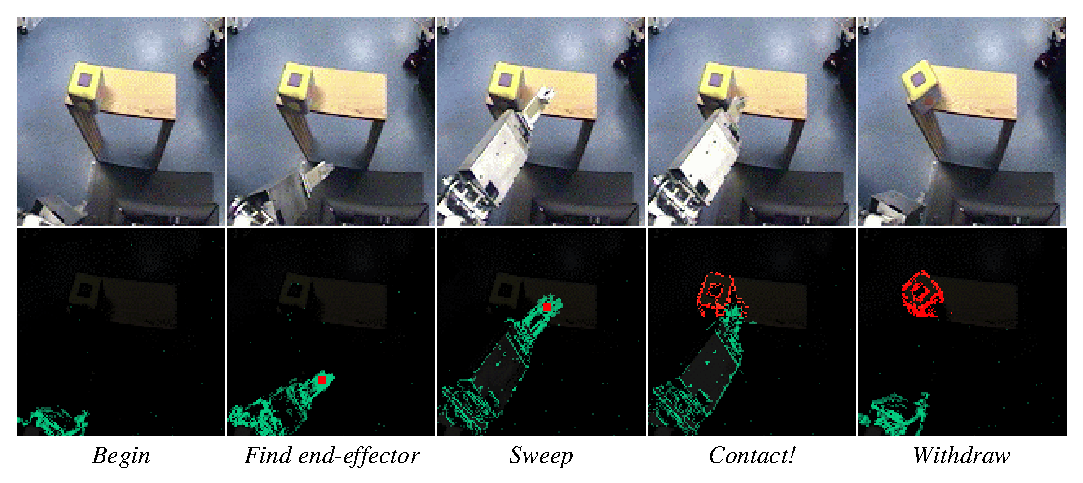
\includegraphics[width=\columnwidth]{poking-sequence.eps}

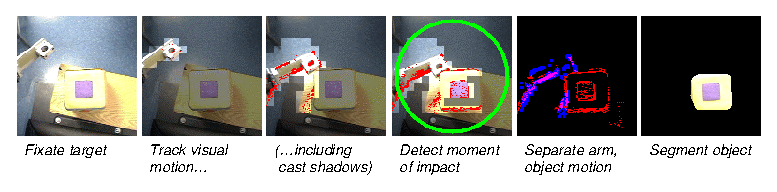
\includegraphics[width=\columnwidth]{fig-poke-zoom.eps}
%%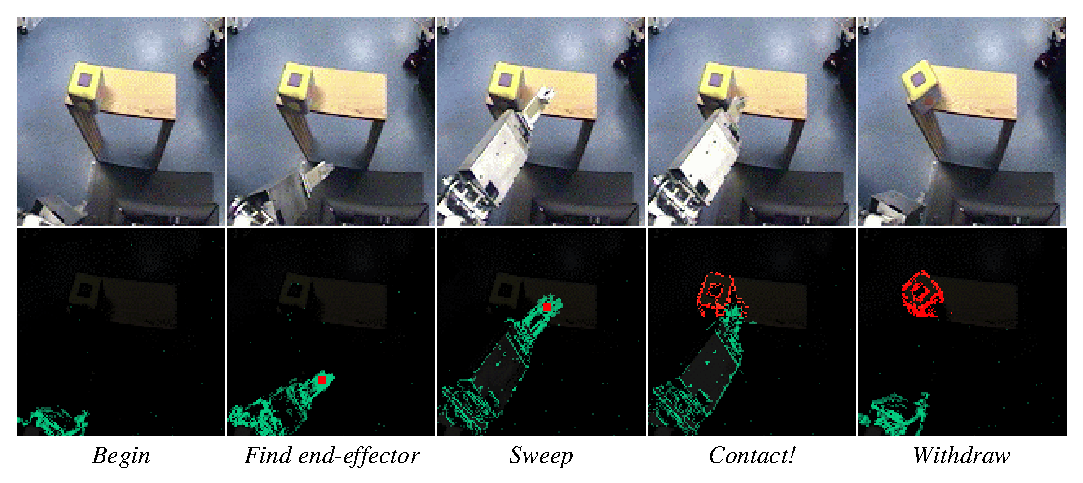
\includegraphics[width=\textwidth]{poking-sequence.eps}
%%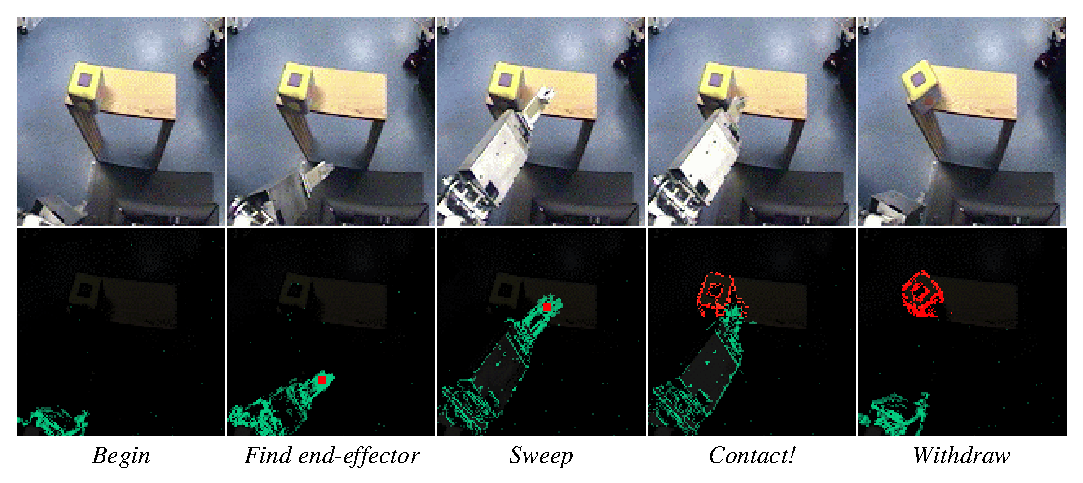
\includegraphics[width=14cm]{poking-sequence.eps}
\caption{ 
\label{fig:poking-sequence}
%
  The upper sequence shows an arm extending into a workspace, tapping
  an object, and retracting.  This is an exploratory mechanism for
  finding the boundaries of objects, and essentially requires the arm
  to collide with objects under normal operation, rather than as an
  occasional accident.  The lower sequence shows the shape
  identified from the tap using simple image differencing and flipper
  tracking.
%
}
\end{center}
\end{figure}



\section{Perceiving actions on objects}

When the arm enters into contact with an object, one of several
outcomes are possible.  If the object is large, heavy, or otherwise
unyielding, motion of the arm may simply be resisted without any
visible effect.  Such objects are of little interest, except in their
role as obstacles, since the robot will not be able to manipulate
them.  But if the object is smaller, it is likely to move a little in
response to the nudge of the arm.  This movement will be temporally
correlated with the time of impact, and will be connected spatially to
the end-effector -- constraints that are not available in passive
scenarios~\cite{birchfield99depth}.  If the object is reasonably
rigid, and the movement has some component in parallel to the image
plane, the result is likely to be a flow field whose extent reflects
the physical boundaries of the object.  This visible response to
the robots action can be used to refine its model of the object's
extent, which may be inaccurate.  For the example scene in
Figure~\ref{fig:setup-sequence} (a cube sitting on a table), the small
inner square on the cube's surface pattern might be selected as a
target.  The robot can certainly reach towards this target, but
grasping it would prove difficult without a correct estimate of the
object's physical extent.  In this section we show how the robot can
experimentally determine an object's extent using the same idea of
correlated motion used earlier to detect its own arm.

Figure~\ref{fig:poking-sequence} shows how a ``poking'' movement can
be used to refine a target.  During a poke operation, the arm begins
by extending outwards from the resting position.  The end-effector (or
``flipper'') is localized as the arm sweeps rapidly outwards, using
the heuristic that it lies at the highest point of the region of optic
flow swept out by the arm in the image (the head orientation and
reaching trajectory are controlled so that this is true).  The arm is
driven outward into the neighborhood of the target which we wish to
define, stopping if an unexpected obstruction is reached.  If no
obstruction is met, the flipper makes a gentle sweep of the area
around the target.  This minimizes the opportunity for the motion of
the arm itself to cause confusion; the motion of the flipper is
bounded around the endpoint whose location we know from tracking
during the extension phase, and can be subtracted easily.  Flow not
connected to the end-effector can be ignored as a distractor.
Figure~\ref{fig:poking-segmentation} shows more detailed results,
including examples of the actual segmented region assigned to the
object.  In the absence of strong texture there may be little motion
signature in the interior of the object, so we recruit a maximum-flow
algorithm due to \cite{boykov01experimental} to fill in such regions
efficiently.

\ifverbose
For simplicity, the head is kept steady throughout the poking
operation, so that simple image differencing can be used to detect
motion at a higher resolution than optic flow.  Because a poking
operation currently always starts from the same location, the arm
is localized using a simple heuristic rather than the procedure described
in the previous section -- the first region of optic flow appearing
in the lower part of the robot's view when the reach begins
is assumed to be the arm.
\fi

\ifverbose
\begin{figure}[tbh]
\begin{center}
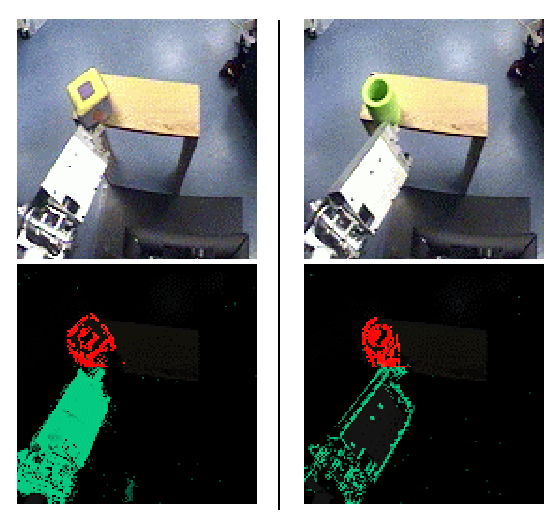
\includegraphics[width=\columnwidth]{cube-and-cylinder.eps}
\caption{ 
\label{fig:cube-and-cylinder}
%
  Poking can reveal a diffence in the shape of two objects without
  any prior knowledge of their appearance.
%
}
\end{center}
\end{figure}
\fi

The poking operation gives clear results for a rigid object that is
free to move.  What happens for non-rigid objects and objects that are
attached to other objects?  Here the results of poking are likely to
be more complicated to interpret -- but in a sense this is a good
sign, since it is in just such cases that the idea of an object
becomes less well-defined.  Poking has the potential to offer an
operational theory of ``objecthood'' that is more tractable than a
vision-only approach might give, and which cleaves better to the true
nature of physical assemblages.  The idea of a physical object is
rarely completely coherent, since it depends on where you draw its
boundary and that may well be task-dependent.  Poking allows us to
determine the boundary around a mass that moves together when
disturbed, which is exactly what we need to know for manipulation.  As
an operational definition of object, this has the attractive property
of breaking down into ambiguity in the right circumstances -- such
as for large interconnected messes, floppy formless ones, liquids,
and so on.

%
\begin{figure}[tb]
\begin{center}
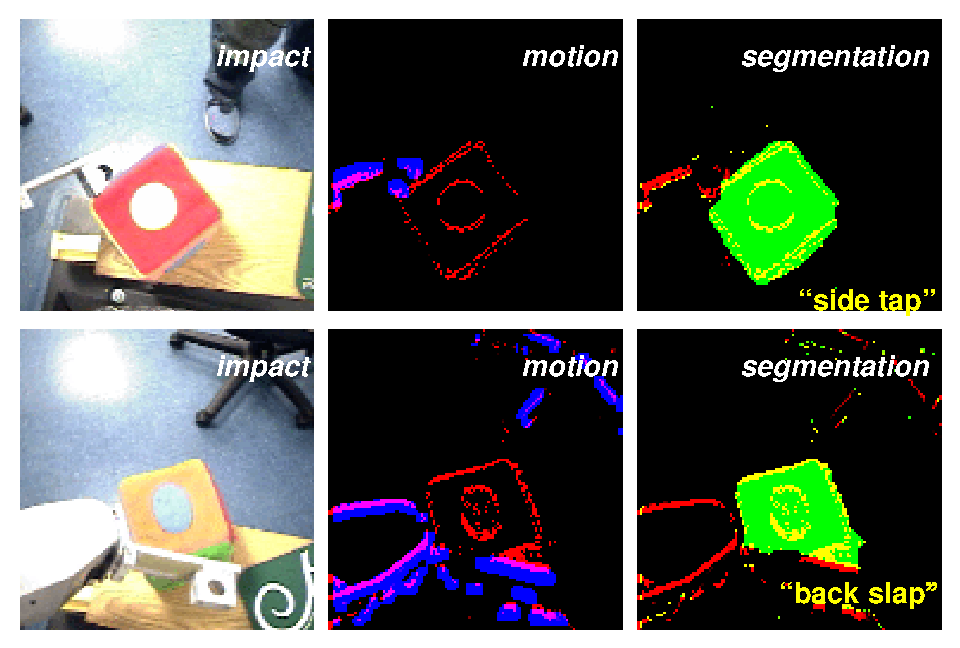
\includegraphics[width=8cm]{segmentation-detail.eps}
%%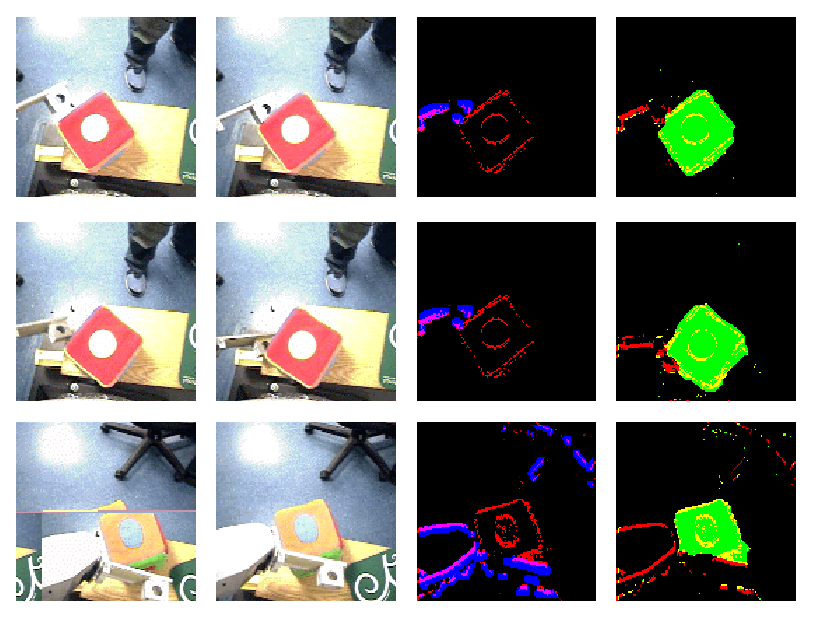
\includegraphics[width=\columnwidth]{poking_segmentation.eps}
\caption{ 
\label{fig:poking-segmentation}
%
Cog batting a cube around.  The top two rows show the flipper poking
the object repeatedly from the side, turning it slightly.  The third
row shows Cog batting an object away.  The images in the first column
are frames prior to a collision.  The second column shows the actual
impact.  The third column shows the motion signal at the point of
contact.  The bright regions in the images in the final column show
the segmentations produced for the object. 
%
}
\end{center}
\end{figure}
%

